%!TEX root = ../template.tex
%%%%%%%%%%%%%%%%%%%%%%%%%%%%%%%%%%%%%%%%%%%%%%%%%%%%%%%%%%%%%%%%%%%%
%% chapter4.tex
%% NOVA thesis document file
%%
%% Chapter with lots of dummy text
%%%%%%%%%%%%%%%%%%%%%%%%%%%%%%%%%%%%%%%%%%%%%%%%%%%%%%%%%%%%%%%%%%%%

\typeout{NT FILE chapter4.tex}%

\chapter{Background}
\label{cha:background}

\section{Microservices} % (fold)
\label{sec:microservices}

Microservices \cite{microservices, microservices2017tenets, microservicesTomorrow} are an architectural style in which software is developed using self-contained components that
communicate with one another via standardized network interfaces.
These services segregate fine-grained business functionalities and can be independently tested, deployed, and scaled by automated mechanisms.
There is typically no centralized management, each service may be written in a different programming language and employ a different data storage technology.

To understand the microservice style it's useful to compare it to the monolithic style:
Monolithic application's are built often using the Model-View-Controller (MVC) pattern~\cite{mvc}, which is composed by three parts:
The view, a client-side user interface composed of HTML pages and Javascript that runs in the user's browser;
The model, a relational database management system;
The controller, a server-side application that handles requests, retrieves and updates data from the database, executes domain logic,
and populates the views that are sent to the browser.

The server-side application is a monolith, a single logical executable, in which all logic for handling requests runs as a single process,
different domains of the application are divided into classes, functions, and namespaces by utilizing the basic features of a programming language.

Large monolithic software becomes a barrier when the underlying application must scale while maintaining a high level of availability.
Scaling the server-side application involves scaling all the application functionalities, rather than the functionalities that require greater resources.
Any small change involves building and re-deploying the entire monolith.

In contrast to monolithic applications, several techniques are used in the microservice architecture to meet the requirements of system scalability and high availability, namely:

\begin{figure}[htbp]
    \centering
    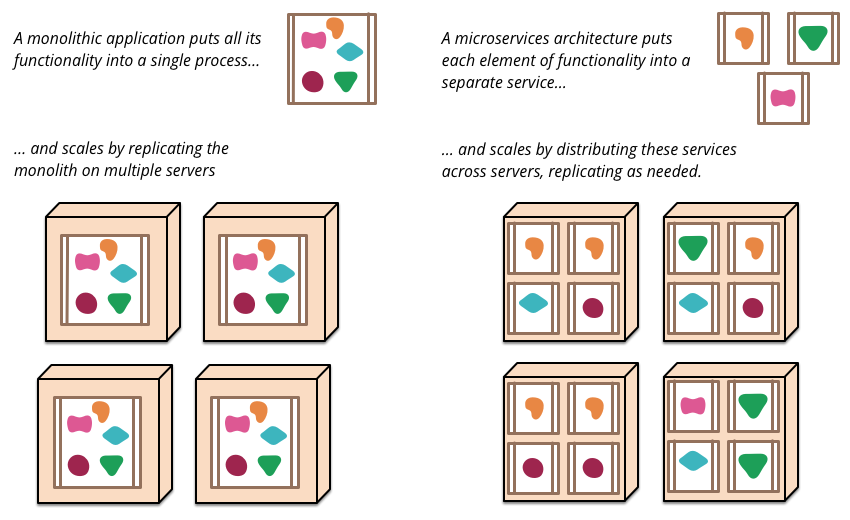
\includegraphics[height=3in]{microVSmono}
    \caption{Monoliths and Microservices \cite{microservices}}
    \label{fig:monoliths and microservices}
\end{figure}

//TODO use description

\paragraph{- Componentization -}

In contrast to monoliths, which achieve componentization solely via the use of libraries and programming language capabilities,
microservices achieve componentization primarily through the division of different business domains and functionalities into distinct executables
that are exposed as services.

While this componentization approach helps to enforce component's encapsulation via more explicit component interfaces,
its primary benefit is that services become independently deployable.

This feature helps to fulfill the requirements of system scalability and high availability by
making different components scalable across multiple nodes and limiting cascading errors via the replication and isolation of components.

\paragraph{- Decentralized Data Management -}

While monolithic applications typically use a single logical database for persistent data, microservices provide greater flexibility, fault tolerance,
and scalability by allowing each service to manage its own database, which can be a different instance of the same database technology or a completely different database system.

Decentralizing data responsibility across services has implications for the implementation of cross-domain operations affecting multiple resources.
The common approach for dealing with the problem of consistency when updating multiple resources in a database system is to use transactions.
A transaction must preserve Atomicity, Consistency, Isolation, and Durability, commonly known as ACID properties.
These properties are more difficult to fulfill in a distributed context than in a traditional database setting, hence developing and maintaining applications that use distributed transactions is notoriously complex.
Microservice architectures advocate for transaction-less service coordination with eventual consistency.
The divergence between different services is addressed with the use of compensating operations instead of transactions.

\paragraph{- Communication Channel -}

\citeauthor{microservices}, a well-known author in the context of microservices, promotes the use of ''smart endpoints'' and ''dumb pipes'' for microservices communication.
Enterprise Service Buses (ESB)~\cite{esb} were previously commonly used in service-oriented architecture (SOA) systems,
and it was common to incorporate orchestration and transformation logic into the communication infrastructure,
making the ''pipe smart''.
This approach had several flaws, the tooling was complex and expensive, and it was difficult to solve problems in production environments.

The reverse approach has been adopted with microservices,
where services own their domain-centric logic ''smart endpoints'' and transport messages via ''dumb pipes''.

\paragraph{- Communication Strategies -}
The majority of communication between microservices is done via request/response-based communication or event-driven messaging.

Request/response-based communication protocols are typically suited for synchronous settings,
where the client contacts one receiver at time and needs the response before it can continue.
In this approach there is a clear control of the flow,
there is a service that plays the role of orchestrator and determines the sequence of operations to be performed in other services.
The HTTP~\cite{http} and RPC~\cite{rpc} protocols are the most widely adopted protocols under this approach.

Event-driven messaging communication protocols are suited for asynchronous settings,
where a client publishes a message to multiple receivers and can process the responses at a later time.
In this approach there is no orchestrator, each service knows their role and what to do based on events that occurred.
The main disadvantage of this strategy is that consistency is not guaranteed when multiple services consume events and one of them fails.
Kafka~\cite{kafka} is the most widely adopted protocol under this approach.

\paragraph{Decomposition}
When designing a software system, it's important to decide how the system is divided into distinct components.
Independent replacement and upgrade-ability are key features to consider when designing a component.
The problems caused by poor division of concerns are alleviated in the context of microservices, because a system's are typically divided into small components with a single responsibility,
whereas in traditional architectures components have wider responsibilities.

To reduce the risk of structural refactors, techniques such as Domain-Driven Design (DDD)~\cite{ddd} are often used.
DDD is a software design approach that decomposes a complex system into multiple autonomous bounded contexts,
where all the software structure (e.g\ methods, classes, variables) match the business domain.
If the business domain is well-defined, the requirements of independent replacement and upgrade-ability can be met by reflecting business correlations in the software structure.

\section{Software Provisioning} % (fold)
\label{sec:software_provisioning}

Two key processes are essential to provision distributed systems:
a method for packaging and isolating services;
a system capable of managing physical hardware to support services.

Services can be isolated using one of two methods: containers or virtual machines (VM).
Containers offer the most efficient solution because, unlike virtual machines, they share the host system's kernel with other containers.
VMs virtualize an entire machine down to the hardware layers, while containers only virtualize the software layers above the operating system level.

Docker \cite{docker} is the most popular container technology. It is built on top of the following kernel systems:
\begin{itemize}
    \item Namespaces: Isolate the kernel resources (e.g.\ processes, filesystem, users, network stacks) used by each container.
    \item Cgroups: Isolate the hardware resources used by each container.
    \item Copy-On-Write File system: Allows several containers to share common data.
\end{itemize}

Additionally, Docker provides a mechanism for packaging code and its dependencies, referred to as container images.
A container image is an executable package of software that contains all the components necessary to run an application: code, libraries, runtime and settings.

The management of services can be accomplished with the use container orchestration technologies.
Container orchestration eliminates many of the manual processes involved in the management of distributed systems.
Some popular options used for the lifecycle management of services are Docker Swarm~\cite{docker2016swarm} and Kubernetes~\cite{kubernetes}.

Kubernetes (K8s) is an open-source container orchestration system that evolved from Google's Borg and Omega projects~\cite{burns2016borg}.
It manages the deployment, management, scaling, and networking of containers of distributed systems across a wide range of environments
and cloud providers.
This means ensuring that all containers used to execute various workloads are scheduled to run on physical or virtual machines,
while adhering to the deployment environment's and cluster configuration's constraints.
Any containers that are dead, unresponsive, or otherwise unhealthy are automatically replaced.
Additionally, Kubernetes also provides a control plane to monitor all running containers.
Kubernetes accomplishes this through a well-defined, high-level architecture that encourages extensibility:

\begin{itemize}
    \item Pod: Encapsulates an application's container (or multiple containers),
    storage resources, has a unique network IP address, and provides configuration options for the container(s).
    \item Service: Is an abstraction that defines a logical set of Pods as well as a policy for accessing them.
    \item Volume: Is a directory which is accessible to the
    Containers in a Pod.
    \item Namespace: Defines the scope of resource names, which must be distinct within the same namespace but not across namespaces.
    \item Deployment: Describes the desired state of the system.
    \item ReplicaSet: Ensures that a certain number of pod replicas are active at all times.
    \item DaemonSet: Ensures that all, or some Nodes are running a replica of a Pod.
    \item StatefulSet: Is used to manage stateful applications.
\end{itemize}

Kubernetes is a more sophisticated container management system than Docker Swarm.
Docker Swarm is only compatible with Docker, whereas Kubernetes is compatible with other container services.
In comparison to Swarm, Kubernetes is more difficult to deploy and manage, however it is more scalable.

\section{DevOps} % (fold)
\label{sec:dev_ops}

DevOps~\cite{devops} can be viewed as a collection of practices designed to accelerate the software development cycle and shorten the time between developing new features and deploying them to production.
The term DevOps is derived from the words development and IT operations, and it refers to the combination and automation of the traditional responsibilities of both departments.

Traditionally the tasks of development, testing, and deployment were divided among different engineering teams.
Different teams had different goals, and in the typical scenario, communication between teams was slow and inefficient.
By automating repetitive operations, DevOps minimizes the need for team coordination and speeds up manual processes that would have taken days or at least several hours.
Building automated pipelines that are executed after the developer changes the codebase is a common DevOps practice.

Pipelines are typically in charge of packaging, testing, and deploying code to testing or production environments.
If any phase of the automated pipeline fails, the developer receives immediate feedback on which task failed, and the pipeline's execution is halted.
An example of a continuous deployment (CD) pipeline is shown in Figure~\ref{fig:pipeline_example}.

\begin{figure}[htbp]
    \centering
    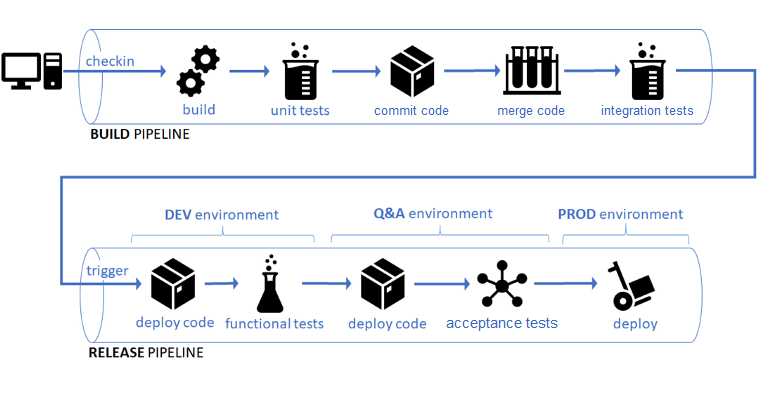
\includegraphics[height=2.9in]{pipelineExample}
    \caption{CD pipeline example}
    \label{fig:pipeline_example}
\end{figure}

The pipeline is divided into two sections the build and release pipelines.
To reduce the iteration time of software development,
the test steps of the build pipeline are conducted first on the developer computer and then repeated and verified on the external pipeline.
The release pipeline entails the deployment of code into production.
The code is initially deployed in staging environments where it is tested and monitored.
After passing all staging phases, the code is considered as part of the system and is deployed into the production environment.

There are less complex pipeline architectures that automate fewer tasks.
A continuous integration (CI) pipeline contains a subset of the tasks of CD pipeline.
It only defines a strategy for continuously integrating and merging code from multiple sources.
Continuous delivery pipeline is an extension of CI, that enables the automation of deployments to staging environments where the software is tested in sequential phases.
A continuous deployment (CD) pipeline goes a step further by defining a strategy for automating the deployment and scaling of software in a production environment.




